% Compile with pdflatex. The editable figure is included below.
\documentclass[11pt,letterpaper]{article}
\usepackage[T1]{fontenc}
\usepackage[utf8]{inputenc}
\usepackage{lmodern,microtype,tikz,hyperref,fancyhdr}
\usepackage[margin=0.88in,headheight=14pt,headsep=12pt]{geometry}
\usepackage[compact]{titlesec}
\definecolor{ink}{HTML}{1C4448}
\definecolor{steel}{HTML}{CBDCDA}
\definecolor{accent}{HTML}{883948}
\hypersetup{colorlinks=true,urlcolor=ink,linkcolor=ink}
\titleformat{\section}{\sffamily\Large\bfseries\color{ink}}{}{0pt}{}
\titleformat{\subsection}{\sffamily\normalsize\bfseries\color{ink}}{}{0pt}{}
\setlength{\parindent}{0pt}
\setlength{\parskip}{0.54em}
\setlength{\emergencystretch}{1.5em}
\pagestyle{fancy}\fancyhf{}\lhead{\small\sffamily NSF AMDO}\rhead{\small\sffamily Initial project description}\rfoot{\small\sffamily Collaborative working draft\quad\thepage}
\begin{document}


\section*{Measurement-Guided Control of Machining Distortion}

A thin aluminum plate can meet its drawing in the fixture and bow out of tolerance when the clamps come off. If enough stock remains on both faces, a machinist can still shift the finished section within the blank while preserving its thickness. The question is when to stop the mill, release the plate and measure its shape while that choice is still available. Measuring too late leaves no room to act. Measuring an easily corrected plate can consume setup time without changing the cut.

\subsection*{Objective and intellectual merit}

We propose to determine when the shape of a partially machined plate reveals which side should supply more of the remaining cut. Two blanks with similar cutting histories can retain different stresses through their thickness. Removing the next layer can then bend them in different directions. Our hypothesis is that, over a measurable range of remaining stock, an observation made after release distinguishes blanks that require opposite allocations. The gain must survive uncertainty from supporting, measuring and reseating the plate.

\begin{center}

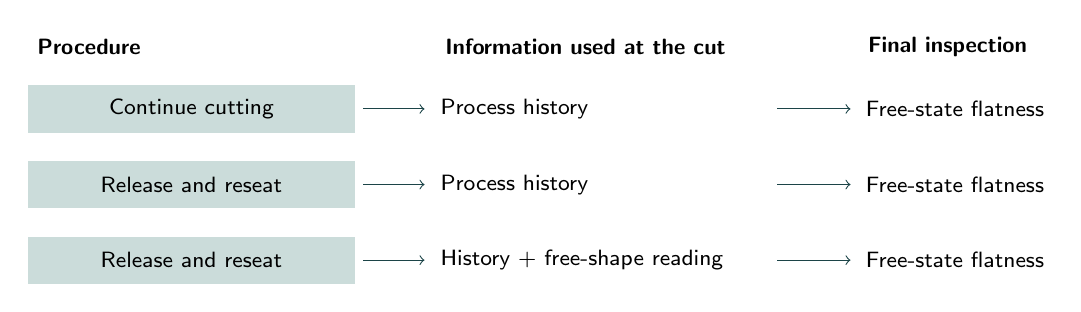
\begin{tikzpicture}[x=1cm,y=1cm,font=\sffamily\footnotesize,every node/.style={align=center}]
\node[anchor=west,font=\sffamily\bfseries\footnotesize] at (0,2.84){Procedure};
\node[anchor=west,font=\sffamily\bfseries\footnotesize] at (5.18,2.84){Information used at the cut};
\node[anchor=west,font=\sffamily\bfseries\footnotesize] at (10.55,2.84){Final inspection};
\foreach \y/\procedure/\rule in {2.05/Continue cutting/Process history,1.09/Release and reseat/Process history,0.13/Release and reseat/History + free-shape reading}{
  \fill[steel] (0,\y-.30) rectangle (4.16,\y+.30);
  \node at (2.08,\y){\procedure};
  \draw[->,ink] (4.26,\y)--(5.04,\y);
  \node[anchor=west] at (5.12,\y){\rule};
  \draw[->,ink] (9.52,\y)--(10.45,\y);
  \node[anchor=west] at (10.52,\y){Free-state flatness};
}
\end{tikzpicture}

\end{center}

{\small\textbf{Figure 1.} The two reseated groups differ only in whether the rule can use the reading. The continuous-cut group establishes the shop baseline for yield and setup time.}

Hao and colleagues already used deformation histories to adjust face allowances in machining trials [1]. Li and colleagues established a geometric limit beyond which a shift cannot recover the part [2]. An NSF GOALI award linked residual-stress estimation with tool-path design [4]. Together these precedents locate the open question precisely. Among blanks with two feasible allocations, how much does one additional observation improve the probability of meeting a drawing, and at what cost in occupied machine time?

\newpage

\section*{Aim 1 · Establish when a release measurement is informative}

% For Satish Bukkapatnam: identify a drawing, candidate fixture, mill operator and gauge.
\textbf{Year 1.} Bukkapatnam’s group will qualify one two-sided milling setup and an independent measurement of final free-state flatness. We will seek an unfeatured plate drawing that allows both face allocations at the same final thickness. Each must leave enough material to clean up both faces [2]. Before committing to cutting trials, we will release and reseat a rough-machined plate repeatedly without cutting, record support locations and temperature, and time the complete interruption. Repeating the free-state scan after repositioning will show whether apparent changes in bow are large enough to distinguish from support and gauge variation.

\subsection*{Learn the effects of the two cuts}

We will cut sibling blanks from known positions in several parent plates and record their depth and orientation. At planned levels of remaining stock, we will measure their relaxed shape and randomly assign a drawing-permitted split within each block. Both assignments will receive the same handling. Sibling blanks let us compare the effects of opposite cuts under similar starting conditions. We will retain signed curvature along a marked direction before finishing and use the drawing’s free-state flatness criterion to judge the finished part.

Zhang’s group will use variation between parent plates to size the validation study. Repeated height readings on a blank characterize measurement uncertainty. Independent parent plates determine how far the result can travel. If the drawing fixes the final mid-plane or both candidate cuts produce equivalent flatness within a practically important margin, we will document the applicable bound and reconsider the case for a larger trial.

\newpage

\section*{Aim 2 · Identify the stock ranges where the reading changes the cut}

% For Rui Tuo: specify the two stress profiles that existing observations cannot distinguish.
\textbf{Year 2.} Tuo’s group will compare a mechanical model driven by inherited through-thickness stresses with an extension that allows the cuts themselves to introduce near-surface stress. Each model will predict the difference in final flatness between two feasible allocations. We will compare their predictions with a history-based allowance rule adapted from Hao and colleagues [1] and a predictor using a reduced set of layer-removal measurements [3]. We will document which signals our fixture can measure and charge each method for the observations it requires.

Predictions will guide the next experiment. We will select stock levels and cutting histories where two explanations fit the existing measurements but favor opposite allocations. Bukkapatnam’s group will machine new sibling blanks at these settings. Zhang’s group will evaluate the prespecified contrasts using independent parent plates, building on the team’s work in physical model validation [6]. A flatness difference smaller than the combined metrology uncertainty will leave the contrast unresolved. The contrast tests which model predicts the better cut. A causal attribution to a stress source would require an independent stress measurement. The same allocation may work across both curvature signs.

\subsection*{Decide whether to interrupt before seeing the reading}

The proposed policy has two decisions. Using only the cutting history and stock still available, it first chooses whether to stop. If it stops, the released shape can then inform the split. During development we will estimate how often the reading changes the preferred split, the expected yield gain and the time it requires. Several distinct ranges may justify interruption. Regions with sparse parent-plate evidence will be marked as uncertain before either rule is frozen.

\newpage

\section*{Aim 3 · Test the decision on independently sourced stock}

% For Xianyang Zhang: specify independent parent lots, a meaningful decision margin and validation sample size.
\textbf{Year 3.} Before model fitting, Zhang’s group will reserve whole parent plates for the final test. Within prespecified stock ranges, we will randomly assign sibling blanks to continuous machining with the history-based rule, to release and reseating with the reading withheld, or to the same handling with the reading available to the allocation rule. We will record the rule’s planned interruption decision before any release. The two reseated groups isolate the value of seeing the reading. The continuous group establishes the net effect of interrupting the job. An independent inspector, blind to assignment, will grade released parts. We will report tolerance yield, continuous flatness and occupied machine minutes with uncertainty across parent plates.

Using the frozen policy’s prespecified stock ranges, we will estimate its gain against continuous machining, including blanks on which it would skip measurement. A result near zero with a wide interval leaves the economics unresolved. If the shop supplies a cost per rejected blank and a machine-hour rate, we will estimate net savings. Otherwise we will report the break-even cost per avoided reject.

\subsection*{Feasibility and broader impacts}

Bukkapatnam’s group has validated motion on an instrumented Langmuir MR-1 CNC mill [7]. Texas A\&M also lists a shared Haas five-axis CNC mill [5]. Either could support the single-mill pilot once an operator, drawing and traceable stock are available. A loaded test cut and an independent flatness gauge will establish whether the setup resolves the drawing tolerance. We will develop a teaching dataset pairing cutting histories, relaxed shapes and blinded final grades. Students will choose whether to interrupt a job and how to allocate stock. Before and after the exercise, students will select policies on held-out cases matched by difficulty. We will compare the choices with a history-only baseline using yield and machine time estimated from randomized sibling groups. Each blank reveals the outcome of its assigned cut.

\subsection*{Selected sources}

\begin{enumerate}
\small\setlength{\itemsep}{0pt}
\item \href{https://doi.org/10.1016/j.cja.2020.03.038}{Hao et al. Online deformation monitoring and machining allowance control.}
\item \href{https://doi.org/10.1016/j.cirp.2015.04.025}{Li et al. Stock allowance and compensation of machining distortion.}
\item \href{https://doi.org/10.3390/jmmp8010009}{Aurrekoetxea et al. Layer removal and the placement of machined parts.}
\item \href{https://www.nsf.gov/awardsearch/showAward?AWD_ID=1762722}{NSF. GOALI project on machining distortion, award 1762722.}
\item \href{https://texasmakes.tamu.edu/facilities/}{Texas A\&M Engineering Experiment Station. Institute for Manufacturing Systems facilities.}
\item \href{https://arxiv.org/abs/2604.17144}{Li, Zhang and Tuo. Physical model validation against observations. Preprint, 2026.}
\item \href{https://ssrn.com/abstract=7243783}{Hanchate et al. Digital Twins for Manufacturing Machine Tools: Architecture and Validation Principles. Preprint, 2026.}
\end{enumerate}

\end{document}
